\newpage
\section{Prac 4 - SPI and Threading}
\subsection{Overview}
While the Pi 3B+ does have an audio jack, it uses a purely PWM (pulse width modulation) based implementation for audio. Audiophiles among you may know that this is not a great way of playing audio. You can read more about the Raspberry Pi and it's audio jack \href{https://hackaday.com/2018/07/13/behind-the-pin-how-the-raspberry-pi-gets-its-audio/}{here}.

To improve audio quality, we can use a DAC (digital to analog converter). 

\subsection{A Very Short Introduction to Digital Audio}
\textit{If you'd like to better understand the basics of audio quality, I suggest reading \href{https://medium.com/@MicroPyramid/understanding-audio-quality-bit-rate-sample-rate-14286953d71f}{this article}. If you find any of this interesting even in the slightest), or you're interested in signal processing, I strongly suggest the DSP course in fourth year.}

Sound waves are continuous waves in time. Unfortunately, we can't represent continuous waves in digital systems. Instead, we take discrete samples of the continuous waves at a specific interval (with help from Nyquist) to be able to reconstruct the wave to the best of our ability. This rate is called the \textit{sample rate}. You may recognise common audio sample rates, such as 44.1kHz, which is standard CD quality.

Figure \ref{fig:Signal_Sampling} below\footnote{By Email4mobile (talk) http://en.wikipedia.org/wiki/File:Signal\_Sampling.png, Public Domain, https://commons.wikimedia.org/w/index.php?curid=8693098} shows the difference between the continuous and discrete representations. The sampling interval is represented by the value \textit{T}. From basic physics, we know that $f = \frac{1}{T}$. So if we're using a CD for playback, we can determine the sampling period, T, to be $T = \frac{1}{f} \approx 22.7 \mu S$.

\begin{figure}[H]
\centering
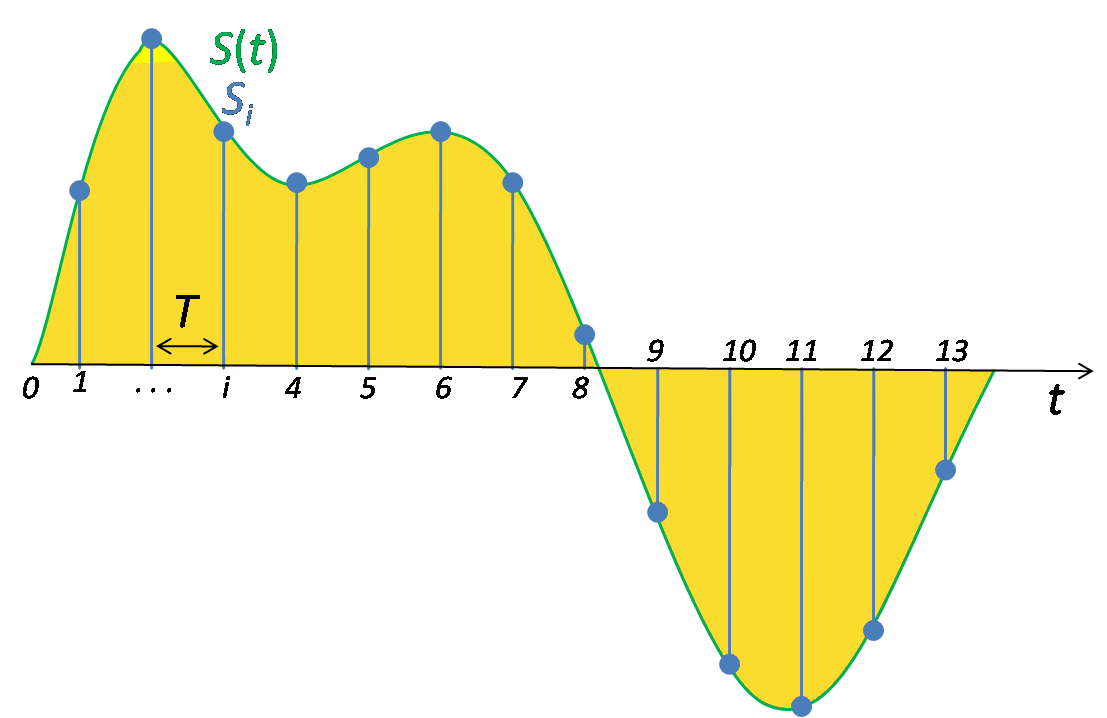
\includegraphics[width=0.6\columnwidth]{Figures/Signal_Sampling}
\caption{Signal sampling representation. The continuous signal is represented with a green coloured line while the discrete samples are indicated by the blue vertical lines.}
\label{fig:Signal_Sampling}
\end{figure}

Recall from Prac 2, where we spoke about about bit widths. The greater the bit width, the more accurate our number. Now consider the DAC we're using the MCP4911. It is a 10 bit DAC, meaning we have 10 bits to work with. If you recall from your lectures, it means we can split the voltage outputs into 10 distinct levels. CD quality uses 16 bits.

Our practical uses 8 bit 16kHz audio - the lowest possible quality we could make! This is purely because we're using a cheap DAC. So unfortunately the audio you will get at the output will sound worse than what you might expect from a song - but it won't sound much different from if you had to play the same file through a high end audio system. What's important to take away from this practical is an introduction to SPI, and some knowledge about audio, hard time constraints, and an appreciation that the Raspberry Pi may not always be the best choice for your application. 

Audio processing has a hard time requirement. This means that the audio events need to happen at a very specific time with no variations. Because the Raspberry Pi uses a Linux based operating system, there's no ability to for it to perform hard time operations. Instead it performs the operations to the best of it's ability. 

Because audio is a hard time constraint, we need to make sure that samples are ready to play as soon as they are requested. To do this, we use a technique called "circular buffering". Correct and complete implementation of a circular buffer can get tricky, so in this practical we're mimicking it by using a single array split into two parts. As the one half of the buffer (array) loads, the other half plays. We need to put measures in place to ensure that we don't write over data we are yet to play, or try and play from the buffer before any audio samples have been written to it. Because our Pi operates faster than we need the audio to be played out over SPI, we're mostly okay, but to be safe we're going to implement these checks anyway. The buffer size that is set has consequences, too. Too small a buffer size, and the audio playback will experience "popping". Too large, and we use too much memory. For this practical, a total buffer size of 1000 samples should be sufficient.


\subsection{Pre-prac requirements}
This section covers what you will need to know before starting the practical.
\begin{itemize}
    \item Read the \href{http://ww1.microchip.com/downloads/en/DeviceDoc/22248a.pdf}{MCP4911 Datasheet} and understand the registers and what each bit represents (see page 24).
    \item Revise bit shifting in C/C++ from ES I
    \item Read the WiringPi documentation on SPI
\end{itemize}

\subsection{Outcomes}
You will learn about the following aspects:
\begin{itemize}
    \item Reading from an external file
    \item SPI
    \item Threading
\end{itemize}

\subsubsection{Pre-prac Submissions}
A circuit diagram for the practical. You will need to upload a schematic detailing how you are going to set up the DAC and connect it to the Raspberry Pi. It should also show how the buttons are connected to the Pi. Software used for drawing the circuit is up to you. \footnote{You should be aware that Wiring Pi has 3 different potential modes for pin usage. Be aware of that during config and your wiring.}

\subsection{Deliverables}
At the end of this practical, you must:
\begin{itemize}
    \item Demonstrate your working implementation to a tutor
    \item Submit your report on Vula
\end{itemize}

\subsection{Hardware Required}
\begin{table}[H]
\begin{tabular}{ll}
\begin{tabular}[c]{@{}l@{}}\tabitem Configured Raspberry Pi \\ \tabitem RPi Power Source (power brick)\\ \tabitem Ethernet Cable\\ \tabitem A breadboard \end{tabular} & 
\begin{tabular}[c]{@{}l@{}}\tabitem 2 x push buttons\\ \tabitem MCP4911 DAC\\ \tabitem Dupont Wires\\ \tabitem A set of earphones  \\\end{tabular}  
\end{tabular}%
\end{table}

\subsection{Further Instructions}
\begin{itemize}
    \item If you didn't in Prac 0, enable SPI in raspi-config
    \item Fetch the updated Practical code off GitHub by running git pull in the prac source, and move it in to your own folder to work with. This is a tricky practical and use of git (not necessarily GitHub) is strongly recommended for this practical
    \item Read through the code that is given to you, and try and understand what you are still required to do. be aware that you need to make changes to Prac4.h
    \item Start by writing your initialisation. You need to determine the rate at which the audio plays by setting the SPI Clock. You should also be aware that the Raspberry Pi isn't that great at holding an SPI clock. There is occasionally a scaling factor of 8/5 in the SPI clock due to the fact that the SPI clock comes from the CPU clock, which changes depending on load.\footnote{Note that this factor isn't constant - sometimes the Pi might actually run at the clock rate you give it. To resolve this issue, you can force a stable clock rate on the CPU, but that isn't necessary for this practical. Testing tells me that the Pi is more likely to downclock, requiring us to need that factor. If you want to be certain, hook the SPI clock pin out to an oscilloscope}$^,$\footnote{Understand why \href{https://github.com/raspberrypi/linux/issues/2094}{here}}. So if you want a 16kHz SPI clock, you need to multiply that by 8/5 and tell the Wiring Pi library to use a clock of 25.6kHz. You can use the formula $SPICLOCK = SAMPLE RATE * WIDTH * No. CHANNELS * 8/5$ to determine the SPI clock you need. Recall width here refers to the total number of bits to be transferred for a single sample (16 bits).
    \item Write code to read in the file to the buffers. The file that you have been provided with is a 16kHz, 8 bit .raw file. This makes it simple for the sound to be processed as all that needs to be done is to read in each 8 bit character and send it to the DAC. Make sure you understand how the buffering is working.
    \item Create the code that plays audio over SPI to the DAC. It's a good idea to give this thread a high priority. You can read about thread priorities \href{https://docs.oracle.com/cd/E19455-01/806-5257/attrib-16/index.html}{here}.
    \item Create the two interrupts you require to pause playback, and stop playback. Stop playback could be considered as an "exit" as well. Pause should stop playback and reading from the buffer when first pressed. When pressed again, playback should continue.
    \item You can listen to the output of the DAC on earphones (given that you're passing the correct control bits). Otherwise, you need to pass it through an amplifier.\footnote{You probably don't want to do this as the audio quality is so low in this prac.}
    \item You need to demo playback, pause/play and stop to a tutor in a demo. They will examine your code to ensure you've used threading and interrupts.
\end{itemize}

\subsubsection{Report Instructions}
Your three page write up should consist of the following headings:
\begin{enumerate}
    \item Introduction\\
    Describe the prac (what you're doing and how you're doing it) [0.5-1 pages]
    \item SPI communication using Wiring Pi [0.5 pages]
    \begin{enumerate}
    \item Initialisation, including the clock speed calculation
    \item Send data
    \end{enumerate}
    \item A few sentences highlighting the importance of real time constraints, and why the Raspberry Pi (under Raspbian) is unable to implement these. [0.5 pages]
    \item The circuit diagram from the pre-prac, with any changes you've made updated in the circuit diagram [0.5-1 pages]
\end{enumerate}


